\documentclass{article}
\usepackage{thomaspackage}
\usetikzlibrary{matrix}

\begin{document}
	\tableofcontents
	\section{Sommen}
 		Onthoud:
 		\begin{align*}
 			\sum_{k=c}^{\infty} r^k &= \frac{r^c}{1-r} \\
 			\sum_{k=1}^{\infty} \frac{1}{k^2} &= \frac{\pi^2}{6} \\
 			\sum_{k=0}^\infty \frac{x^k}{k!} &= e^x \\
 		\end{align*}
 		
 		Uit de eerste kunnen we andere sommen afleiden. bijvoorbeeld 
 		$\displaystyle \sum_{k=0}^{\infty} kr^k: $
 		\begin{align*}
 				\sum_{k=0}^{\infty} r^k &= \frac{1}{1-r} \text { differenti\"eren aan beide kanten } \to \\
 				\sum_{k=0}^{\infty} kr^{k-1} &= \frac{1}{(1-r)^2} \\
 				\sum_{k=0}^{\infty} kr^k &= \frac{r}{(1-r)^2} \\
 		\end{align*}
 		Op dezelfde manier $\displaystyle \sum_{k=1}^{\infty} \frac{1}{k2^k}$:
 		\begin{align*}
 				\sum_{k=0}^{\infty} r^k &= \frac{1}{1-r} \text { integreren aan beide kanten } \to \\
 				\sum_{k=0}^{\infty} \frac{1}{k+1} r^{k+1} &= -\log_e (1-r) \\
 				\sum_{k-1}^\infty \frac{1}{k} r^k &= \log_e (\frac{1}{1-r})
 		\end{align*}
 		Eindig sommen kunnen we nu ook:
 		\begin{align*}
 			\sum_{k=c}^n r^k &= \sum_{k=c}^\infty r^k - \sum_{k=n}^\infty r^k
 		\end{align*}
 		
 	\section{Integralen}
	 	\begin{stelling}[Limiet door de integraal halen]
		 	Zij $\f_k,\f \: \reals^n \to \reals$, met $\lim_{k \to \infty} \f_k = \f$, dan
		 	\[ \f_k \text { \textbf{convergeert uniform} naar } \f \implies \lim \int \f_k = \int \lim \f_k = \int \f \,. \]
	 	\end{stelling}
	 	
	\section{Partieel integreren}
		\[ 
			\int_a^b f(x) g'(x) \d x = \big[f(x)g(x)\big]_a^b - \int_a^b f'(x) g(x) \d x
		 \]
		 dus kies $f$ en $g$ zodanig dat $f'(x)g(x)$ makkelijk integreert.
 			 
	 \section{Gonioformules}
		 Onthoud:
 		 \begin{align*}
 			 \cos (2\alpha) &= \cos^2 \alpha - \sin^2 \alpha \\
 			 \sin (2\alpha) &= \cos \alpha \sin \alpha 
 		 \end{align*}
 		 
 		 Mocht je iets willen integreren met $\cos^2$ dan volgt uit de eerste regel
 		 \begin{align*}
 		 		 \cos (2\alpha) &= \cos^2 \alpha - \sin^2 \alpha \\
 		 		 &=  \cos^2 \alpha + \cos^2 \alpha - \cos^2 \alpha - \sin^2 \alpha \\
 		 		 &= 2\cos^2 \alpha -1
 		 	 \end{align*}
 		 	 en evenzo voor $\sin^2$.
	 \section{Co\"ordinaten}
		 Bij cilindercoordinaten is een extra \textbf{factor $\bm r$} verplicht als je integreert, bij bolcoordinaten $\rho^2 \sin \phi$
		 
		 Om bolco\"ordinaten te onthouden, gebruik poolco\"ordinaten en druk $r$ uit in $\rho$ en $\phi$ met behulp van onderstaand driehoekje, zodat $r=\rho \sin \phi$, en vul deze in, in poolco\"ordinaten $r \cos \theta,r \sin \theta$ om $x$ en $y$ te krijgen. Vind de $z$-co\"ordinaat op dezelfde manier zodat $z=\rho \cos \phi$.
		 					
		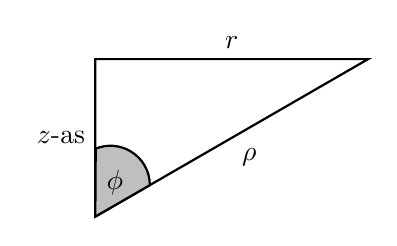
\begin{tikzpicture}[thick]
		\draw(0,0) 
		-- (90:2cm) node[midway,left]{$z$-as} 
		-- (30:4cm) node[midway,above]{$r$} % node of point
		-- (0,0) node[midway,below right]{$\rho$};
		\draw[fill=lightgray, thick] (0,0) 
		-- (30:0.8cm) arc (0:112:0.5cm) node at (60:0.5cm) {$\phi$} 
-- cycle;
		
		\end{tikzpicture}

	\section{Determinant}

		\[
			\det{
				a & b & c \\
				d & e & f \\
				g & h & i \\
			}
			= a \det{e & f \\ h & i} - b \det{d & f \\ g & i} + c \det{d & e \\ g & h}
		\]
		\textbf{Let op het minteken!} Mintekens gaan als volgt:
		\[
			\det{
				+ & - & + \\
				- & + & - \\
				+ & - & +
			}
		 \]
	\section{Inproduct/uitproduct}
		\paragraph{Inproduct (dot product)}
		\[ \x \bullet \bm \phi = \vvec{x \\ y \\ z} \bullet \vvec{\phi_1 \\ \phi_2 \\\phi_3} = x \phi_1 + y \phi_2 + z \phi_3 \]
		\paragraph{Uitproduct (Vector/Cross product)}
		\[ \vvec{x \\ y \\ z} \times \vvec{\phi_1 \\ \phi_2 \\\phi_3} = \vvec{y \phi_3 - \phi_2 z \\ z \phi_1 - \phi_3 x \\ x \phi_2 - \phi_1 y}  \]
		eventueel te onthouden door (zie \LaTeX\ comments)

		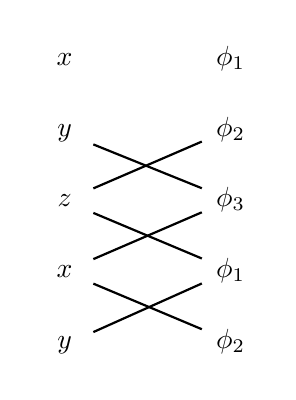
\begin{tikzpicture}[thick]
		\matrix (m) [matrix of math nodes, row sep = 1em, column sep = 4 em, minimum width=2em]
		{
			x & \phi_1 \\
			y & \phi_2 \\
			z & \phi_3 \\
			x & \phi_1 \\
			y & \phi_2 \\
		};
		\path[-stealth]
			(m-2-1) edge[-] (m-3-2) % y keer phi_3
			(m-2-2) edge[-] (m-3-1) % min phi_2 keer z,
			(m-3-1) edge[-] (m-4-2) % z keer phi_1
			(m-3-2) edge[-] (m-4-1) % min phi_3 keer x,
			(m-4-1) edge[-] (m-5-2) % x keer phi_2
			(m-4-2) edge[-] (m-5-1) % min phi_1 keer y
			;
		\end{tikzpicture}
	\section{Bol}
		Inhoud is $\frac{4}{3} \pi r^3$, neem afgeleide voor oppervlakte.
\end{document}